\section{GWAS of left ventricular trabeculation}
\label{section:GWAS_FD}
Early in mammalian heart development, the myocardium is composed of a loose network of fibers and sinusoids that forms sheet-like protrusions into the cardiac lumen. These structures in the inner layer of the myocard will give rise to the trabecular myocardium. In subsequent stages of heart development, the sinusoids disappear and the trabecular myocardium becomes more compacted towards the outer wall of the myocard, forming a thick, compact ventricular wall \citep{Chen2009,Yousef2009}. Failure of the myocardial compaction process leads to persistence of ventricular hypertrabeculation or non-compaction (NC). The majority of NC phenotypes are observed in the left ventricle (LV) \citep{Zambrano2002}. It remains unknown whether LVNC is a distinct disease or a shared characteristic of different cardiomyopahties \citep{Captur2013}. In addition to NC as a clinical phenotype, variation in trabeculation pattern and strength have also been observed in healthy volunteers from different ethnic backgrounds \citep{Kawel2012,Captur2015}. In this study, we aimed to map genetic variation to LV trabeculation phenotypes. Trabeculation is quantified via fractal analysis, which meassures complex patterns. The phenotype obtained is fractal dimension (FD), a unit-mess measure, that serves as a proxy for the complexity i.e. the level of trabeculation of the endocardial wall. The higher the FD measure, the higher the complexity  of the structure. Genotype to phenotype mapping was achieved by fitting a multi-variate LMM to FD meassurements derived throughout the heart.

\subsection{Data}
\subsubsection{Genotypes}

The genotypes were processed as described in section~\ref{sssec:gentoypes}. 


\subsection{Phenotypes}
Cardiac magnetic resonance (CMR) images were conducted at Hammersmith Hospital, London. The fractal dimensions are derived from standard 2D CMR images. Scout images were obtained and used to plan 2D cine balanced steady-state free precession images in the left ventricular short axis (LVSA) plane from base to apex. Each section had a thickness of 8 mm with a 2 mm gap between sections. On average 10 to 12 images were recorded per individual \citep{DeMarvao2014}. Fractal analyses was automised according to the processing pipeline proposed by Captur and colleagues \citeyearpar{Captur2013}. In brief, the images were binarised into blood pool and myocard and the endomyocardial border was extracted via edge detection. The FD was determined by placing grids with known spacing (scale) of increasing size (i.e. increasing number of edges) on the image and counting the number of boxes with non-zero pixels, i.e. how many boxes contain at least one pixel of border. The slope of the linear regression of the log transformed scale versus the log transformed counts corresponds to the FD \citep{Captur2013}.

\subsection{ADAMTSL1 locus is associated with left ventricular trabeculation in healthy individuals}
The FD measurements across the heart were summarized as maximal apical (towards the tip of the heart) and basal FD in analogy to studies by Captur and colleagues \citeyearpar{Captur2013,Captur2014}. The maximal apical and basal FD measurements were modeled jointly with the number of CMR slices per individual in an any effect mt-LMM-GWAS (Equation~\ref{eq:lmm-mv}), including sex, age, height and weight as covariates. Preliminary results are depicted in Figure~\ref{fig:manhattanFD}, where an association with these phenotypes can be observed on chromsome 9. The SNP is an intron variant of the ADAMTSL1 gene.

\begin{figure}[hbtp]
	\centering
	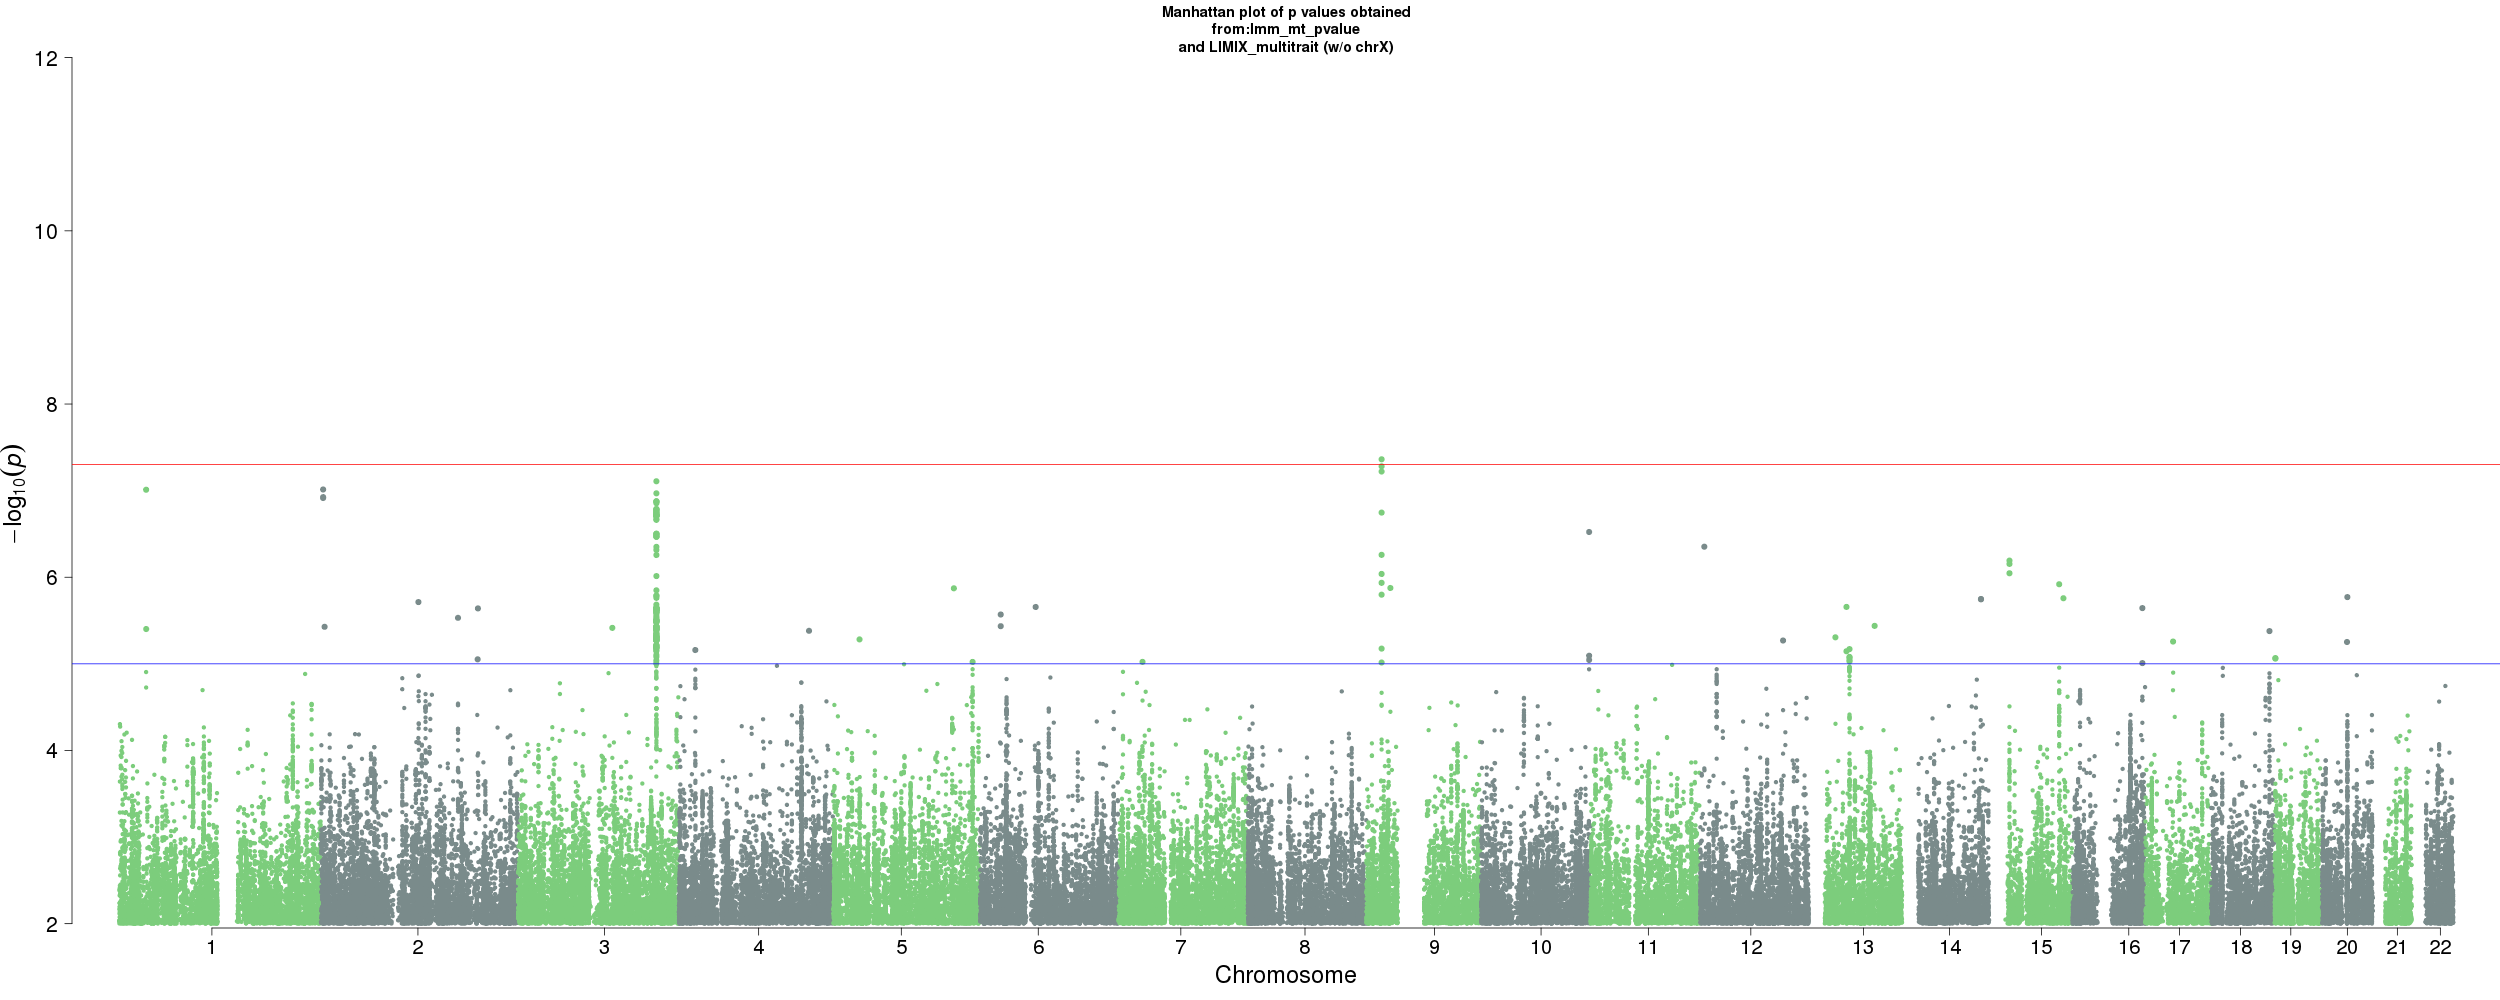
\includegraphics[trim = 0mm 0mm 0mm 100mm, clip, width=1\textwidth]{Figures/lmm_mt_pvalue_LIMIX_multitrait_manhattanplot.png}
	\caption{\textbf{Manhattan plot of genome-wide trabeculation phenotype associations.} Number of CMR slices, maximal apical and basal FD were modeled jointly in an any effect mt-LMM-GWAS with sex, age, height and weight as covariates.}
 	\label{fig:manhattanFD}
\end{figure}

\subsection{Further work}
\begin{itemize}
\item manual QC of genotype cluster plots of SNPs with p-value of less then $5e-4$
\item analysis of ADAMTSL locus for biological function in relation to trabeculation
\item locus zoom of the genomic region
\item potentially improving the presentation of the FD phenotypes to the multi-trait analysis: additional covariates and combinations of the FD measurements
\item replication with UKBiobank data: FD measurements from 2d CMR images scans (access already granted and measurements currently in QC by collaborators)
\end{itemize}
